\section{Internship Internal Project Deployment Phase}
After completing the training phase, I was deployed to the internal project. This section will delve into the specifics of the Internal Project Deployment Phase.

\subsection{Overview}
The internal project, specifically referred to as the internal Billing Tracking Tools Project (a web application), aims to assist administrators in monitoring employee effort lists, planning resources, and generating reports. When using this web application, administrators can upload the billing excel file to the system, then all billing information will be stored in a database server. Administrators can then monitor the billing information, allocate resources (planning), filter the data, and export reports. \\

\noindent During the internal project phase, I was assigned to a team comprising two other members to initiate, develop, and maintain this project. In my capacity as the team leader, I was responsible for overseeing operations, delegating tasks, and tracking the progress of all team members. Concurrently, in my role as a backend developer, I was consistently involved in the development and implementation of all functionalities of the web application.

\subsection{Responsibility}

    \subsubsection{Requirement analysis}
    The requirements analysis process is a phase of the software development process used to explore and analyze project requirements before a project progresses to the software development process phase. \cite{requirement_analysis}. I carefully gathered all the requirements and analysed them.

    \begin{itemize}
        \item \textbf{Identify the users:} The administrator, department manager, project manager
        \item \textbf{Define project objectives:} Build a web application which assists administrators in monitoring employee effort lists, planning resources, and generating reports 
        \item \textbf{Capture and analyse users' requirements: } With the initial sets of user needs and requirements captured, our team created visual representations of the needs and requirements as part of our analysis to inform the definition of the product requirements and user stories.
    \end{itemize}


    \subsubsection{Task assignments}
    As the team leader of the project, I leveraged the OpenProject platform to manage task assignments efficiently, adhering to the Agile framework. The process encompassed several key steps:
        \begin{enumerate}
            \item \textbf{Sprint Planning:} At the beginning of each sprint, the team convened to conduct a comprehensive sprint planning session. During this meeting, we reviewed the project backlog, prioritized tasks based on project goals and deadlines, and defined the sprint scope. Each task was then broken down into manageable user stories and tasks, ensuring they were clear and achievable within the sprint duration.

            \item \textbf{Task Creation and Detailing:} Once the sprint scope was determined, I created tasks in the OpenProject platform. Each task was detailed with specific descriptions, acceptance criteria, and any relevant attachments or references. This ensured that every team member had a clear understanding of the task requirements and expectations.

            \item \textbf{Assignment of Tasks:} Tasks were assigned based on team members' expertise, workload, and personal development goals. I used OpenProject’s assignment feature to allocate tasks to individual team members. This facilitated accountability and ensured that everyone knew their responsibilities.

            \item \textbf{Setting Priorities and Deadlines:} To maintain focus and ensure timely completion, each task was assigned a priority level and a deadline. This helped the team manage their time effectively and work on the most critical tasks first. OpenProject’s priority and deadline features were instrumental in visualizing the workflow and maintaining project timelines.

            \item \textbf{Daily Stand-Ups:} Daily stand-up meetings were held to discuss progress, impediments, and plans for the day. During these meetings, team members updated the status of their tasks on OpenProject, allowing for real-time tracking of the project’s progress. This practice ensured continuous communication and quick resolution of any issues that arose.

            \item  \textbf{Monitoring and Adjustments: } Throughout the sprint, I continuously monitored the progress of tasks using OpenProject’s tracking tools. Burndown charts, task boards, and status updates provided a clear picture of the sprint’s progress. If any task was at risk of delay, adjustments were made promptly by reallocating resources or re-prioritizing tasks to ensure the sprint goals were met.

            \item \textbf{Sprint Review and Retrospective:} At the end of each sprint, a sprint review meeting was conducted to showcase completed work and gather feedback. Following the review, a retrospective meeting was held to reflect on the sprint process, discuss what went well, what could be improved, and implement actionable improvements for the next sprint. 
        \end{enumerate}

        By systematically using the OpenProject platform in conjunction with the Agile framework, I ensured that task assignments were transparent, efficient, and aligned with the overall project goals. This approach facilitated effective collaboration, timely delivery, and continuous improvement within the team.

    \subsubsection{Set up project source code structure}
     The selection of the Flask framework for web application development is underpinned by several compelling factors. Firstly, Flask offers a lightweight and minimalist approach, facilitating rapid development without imposing unnecessary complexities. This agility is particularly advantageous in scenarios where time-to-market is critical, allowing developers to swiftly iterate and deploy features. Additionally, Flask's modular design empowers developers to selectively incorporate components as needed, fostering a tailored and efficient development process. Moreover, Flask boasts a vibrant ecosystem of extensions and libraries, augmenting its core functionality with a plethora of tools for various requirements, such as database integration, authentication, and RESTful API development. Furthermore, Flask's adherence to the WSGI protocol ensures compatibility with a wide range of web servers, enhancing deployment flexibility. Lastly, its extensive documentation and active community support contribute to a robust knowledge base, enabling developers to troubleshoot issues and innovate effectively. Thus, the choice of Flask as the framework for web application development aligns with considerations of agility, modularity, extensibility, compatibility, and support, collectively fostering a conducive environment for efficient and scalable development endeavours. \\
    
     The project source code structure is given in the below table:
     \newpage

     \begin{longtable}{{|m{4.8cm}|m{9.6cm}|}} 
            \hline
			 \textbf{Module/component name} & \textbf{Description}\\ \hline
			 
			 setup.sh & is used for auto-setting up the project.\\ \hline
			 
			 run.sh & a script which runs the web app.\\ \hline
			 
			 requirements.txt & necessary Python packages and libraries list for web app runtime. \\ \hline
			 
			README.md & documentations of the project.\\ \hline
			
			etc-web.conf & the configuration file for deploying the web app. \\ \hline
			
			config.py & acts as environment variables list for the web app while it's working (database connection information, static directory location, etc.) \\ \hline
			
			\_\_init\_\_.py & acts as the main file of the web app, it reads the configurations and establish all routes (APIs) \\ \hline
			
			test/ & test component where contains all unit tests (not available in this version 1.1.0) \\ \hline
			
			static/ & static component where contains all frontend modules (html/, css/, js/) and API documents, log files. \\ \hline
			
			routes/ & routes component where contains all routes modules for each feature (provide API route address, parameters, response). \\ \hline
			
			controllers/ & controllers component where contains all controllers modules for each feature. (handle API paramters, logical calculation, redirection) \\ \hline
			
			models/ & models component where contains all models modules for each feature. (retrieve data directly from the database server) \\ \hline
			
			common/ & common component where contains all user-defined functions which could be shared among many other modules. \\ \hline
			
			data/ & data component where stores all input or output data of the web app. \\ \hline
			
			crontab/ & crontab component where contains the crontab scheduler setup scripts for setting up specific seperate jobs outside the web app. \\ \hline
        \caption{Project source code structure} % needs to go inside longtable environment
        \label{tab:projectStructure}
    \end{longtable}

 


    \subsubsection{Database development}
    Based on the requirements and the advantages of MySQL database management system as mentioned in section \ref{Databases management system}, MYSQL was chosen as the main DBMS of the web application.

    \noindent After that, given that MySQL has two widely-used storage engines for storing web application databases: \textbf{MyISAM} and \textbf{InnoDB}, a detailed comparison and analysis were conducted to determine which storage architecture would best suit the project.

    \begin{longtable}{{|m{5cm}|m{5cm}|}}
            \hline
            \multicolumn{1}{|c|}{\textbf{InnoDB}} & \multicolumn{1}{ c|}{\textbf{MyISAM}}\\ \hline
			 ACID compliant & Not ACID compliant\\ \hline
			 Transactional (Rollback, Commit) & Non-transactional\\ \hline
			 Row Level Locking & Table Level Locking \\ \hline
            Row data stored in pages as per Primary Key order & No particular order for data stored. \\ \hline
            Support Foreign Keys & Does not support relationship constraint \\ \hline
     
        \caption{Comparison of InnoDB and MyISAM MySQL Storage Engines \cite{mysql_comparison_storage_engines}} % needs to go inside longtable environment
        \label{tab:MySQL_storageEngines}
    \end{longtable}

    Upon reviewing the comparison table, InnoDB was chosen as the storage engine for the following reasons:

    \begin{itemize}
        \item \textbf{ACID Compliance, Data Integrity:} InnoDB is ACID (Atomicity, Consistency, Isolation, Durability) compliant, ensuring that all database transactions are processed reliably, maintaining data integrity even in the event of system failures.

        \item \textbf{Transactional Support (Rollback and Commit):} InnoDB supports transactional features such as rollback and commit, providing robust mechanisms for managing transactions, which is crucial for maintaining data consistency and integrity.

        \item \textbf{Concurrency and Performance:} InnoDB utilizes row-level locking, which allows multiple transactions to occur simultaneously without locking entire tables. This enhances performance and scalability, particularly in multi-user environments.

        \item \textbf{Ordered Data Storage:} Storing data in primary key order allows for faster and more efficient data retrieval, especially for queries involving primary key lookups.


        \item \textbf{Support for Referential Integrity:} The ability to define and enforce foreign key constraints ensures that relationships between tables are maintained correctly, preventing orphaned records and ensuring data consistency. 
    \end{itemize}


    After that, I proceeded to design the database schemas to meet the project requirements. This phase involved meticulously defining every entity along with its attributes to ensure consistency and optimization. I carefully considered the relationships between entities, implementing appropriate foreign keys to maintain referential integrity. Additionally, I optimized the schema for performance, ensuring efficient data retrieval and storage. This included normalizing the database to eliminate redundancy and improve data integrity, as well as indexing key attributes to speed up query performance. The goal was to create a robust, scalable, and efficient database structure that would support the web application's functionality seamlessly. 
    
    
    % \noindent As a backend developer, I defined all SQL queries and then built Python functions to use them. Here is an example of the table schema of a specific department:


    \subsubsection{Backend development}
    By adhering to the MVC framework and systematically designing blueprints, routes, controllers, models, and common shared functions, the Flask web application is structured for high maintainability, scalability, and clarity. This approach ensures that the codebase remains organized, with a clear delineation of responsibilities, facilitating collaborative development and long-term maintenance.

    \begin{figure}[H]
			\centering
			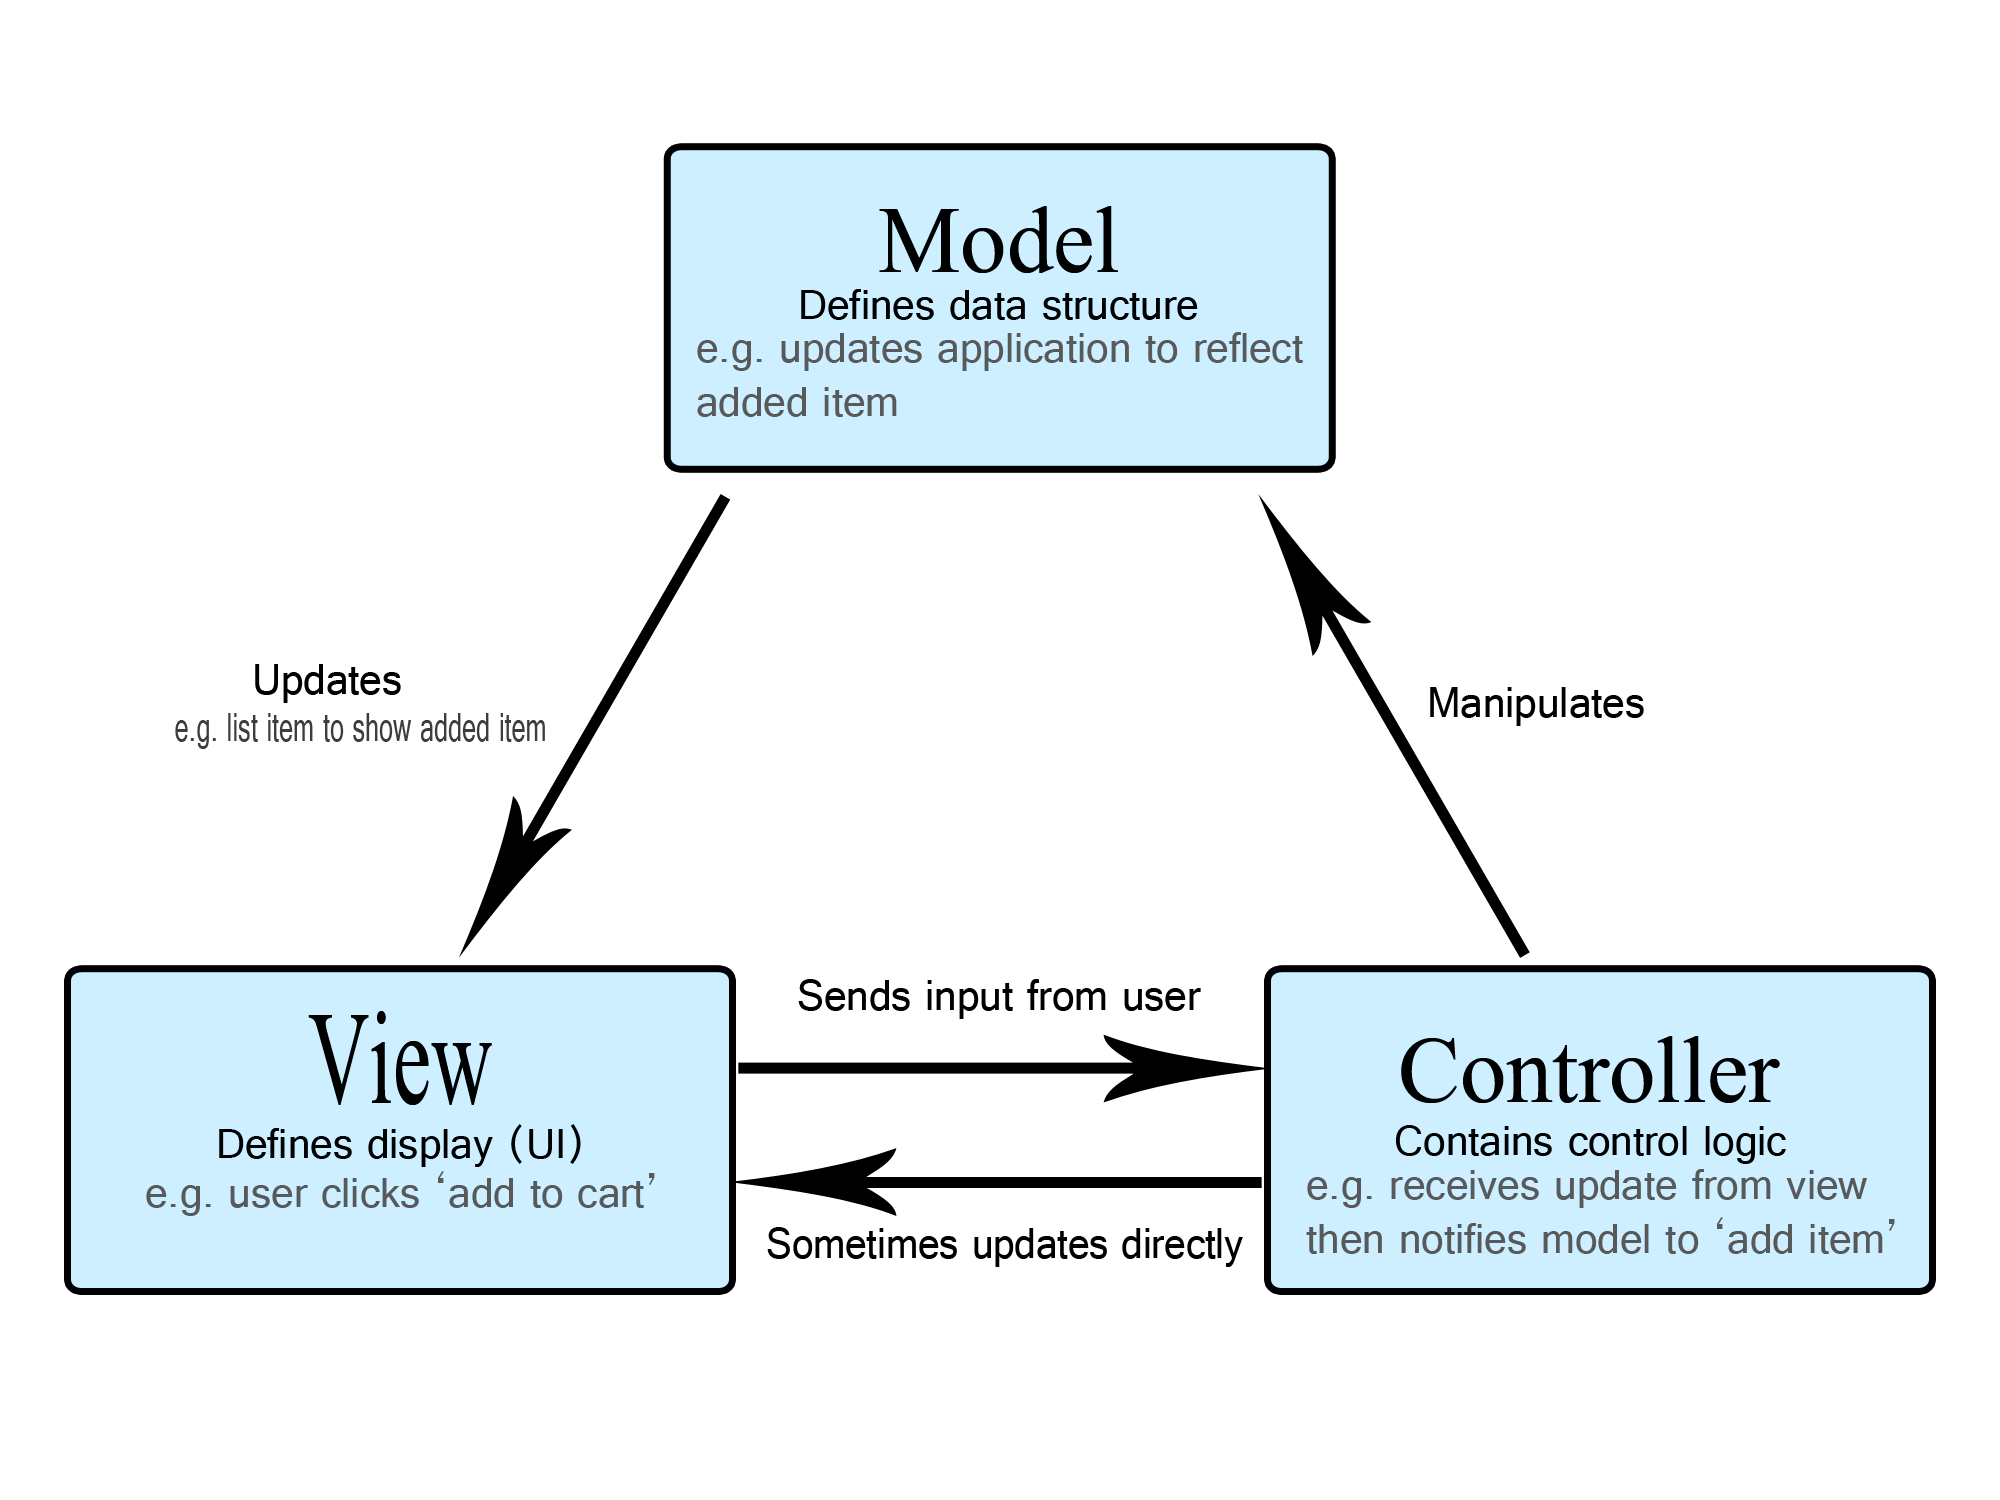
\includegraphics[scale=0.8]{graphics/model-view-controller-light-blue.png}
			\caption{MVC pattern design \cite{mvc}}
			\label{fig:MVC}
	\end{figure}
    
    
    When it comes to designing the application, as a backend developer, I focus on 5 main components below:

    \begin{enumerate}
        \item \textbf{Modular Organization:} Flask blueprints allow the application to be divided into modular components, each representing a distinct feature or functionality. I designed Blueprints to facilitate organized code by grouping related routes, templates, and static files. They are essential for large applications, promoting code reuse and separation of concerns.

        \item \textbf{URL Mapping:} Routes define the URL patterns that the application responds to and associate them with specific controller functions. Flask uses the \textbf{@app.route} decorator together with the corresponding Blueprint to map URLs to view functions. I defined all routes (corresponding to specific endpoints) of the web application, they process requests and generate appropriate responses (Rest API).

        \item \textbf{Logic Implementation:} Controllers contain the core logic for handling requests, interacting with models, and preparing data for views. They validate input, execute business logic, and orchestrate the data flow between models and views. By centralizing the application's logic, controllers ensure a clear separation of concerns.

        \item \textbf{Data Representation:} Models represent 

        \item \textbf{Reusable Components:} Common shared functions include utility functions, helper methods, and services that are used across multiple parts of the application (file utilities, database utilities, etc.). These functions promote code reuse and reduce redundancy. I organized common shared functions into separate packages named \textbf{common/}, which can be imported wherever needed. 
    \end{enumerate}

   My tasks included implementing the API endpoints, encompassing routes, controllers, and models, which provided the necessary data for the frontend. These APIs featured several critical functionalities essential for the web application. Firstly, they facilitated the upload and import of Excel billing files, ensuring seamless data integration. Secondly, the APIs enabled the visualization of billing information, presenting data in an accessible and user-friendly manner. Additionally, they provided robust filtering options to allow users to efficiently search and sort billing information. Another key feature was the generation of report charts, offering graphical representations of billing data for better insights. Lastly, the APIs supported exporting reports, allowing users to download and utilize billing information in various formats for further analysis and record-keeping.

    \subsubsection{Challenges}
    Throughout the web application development, I encountered various challenges that necessitated significant time investment in resolving them, thereby enhancing my technical proficiency.

    \begin{enumerate}
        \item \textbf{Requirement changes: } During the development phase, the requirements for the end-user interfaces and various features have changed. These changes in requirements significantly impacts the scope, timeline, and direction of the project. \\ 
        % Developers must be prepared to handle these changes efficiently and effectively.
        \textbf{\underline{Solution:}} Our team works with stakeholders to prioritize changes based on their impact and feasibility. This helps in focusing on high-value features and prevents the project from becoming overwhelming. Effective scope management ensures that critical requirements are addressed first, while less important changes can be scheduled for later.
        
        \item \textbf{Primary key constraints size limitation:} In the context of database development, the challenge arose from constraints on the size of primary keys imposed by the MySQL DBMS. \\ 
        \textbf{\underline{Solution:}} Consequently, a reassessment of the size allocation for each attribute across database entities became necessary.

        \item \textbf{Concurrency issues:} Another challenge involved concurrency issues arising from simultaneous attempts by users to upload billing excel files while other upload processes were ongoing. Resolving these issues necessitated establishing communication and coordination between these processes. \\ 
        \textbf{\underline{Solution:}} To address this, I implemented a solution using shared files. When an upload process initiates, it creates a file named \textbf{upload\_running}. Upon completion of the upload process, this file is subsequently removed. Therefore, subsequent upload processes are designed to first check for the existence of this file in the system, determining their execution based on its presence or absence.


        \item \textbf{Training for new members:} As a backend developer working on the web application project, introducing new features often necessitates bringing new team members on board to meet deadlines and ensure timely delivery. I had to ensure that new members quickly acquired the necessary knowledge about the project’s architecture, existing features, and coding standards. \\ 
        \textbf{\underline{Solution:}} Creating comprehensive and up-to-date documentation is crucial. This includes detailed architecture diagrams, API documentation, coding guidelines, and setup instructions. A well-maintained knowledge base allows new developers to self-study and reference materials as needed. Additionally, I assigned small and manageable tasks that created a supportive and efficient training environment for new members.
    \end{enumerate}


    \subsubsection{Delivery documentations}
    For the web application project, I have produced two essential documents. The first document details the API specifications using Swagger, ensuring clarity and accessibility in API implementation. The second document encompasses comprehensive guidelines for project requirements, setup procedures, and development practices. These documents aim to streamline communication, facilitate seamless integration of functionalities, and provide clear, structured guidance for efficient project development and deployment.

    

\subsection{Project output}

During my ongoing involvement in the project, I have continued to receive positive feedback from my manager regarding the code structures I have implemented and the maintenance of the project's current flow. \\

\noindent The consistency and usability of the APIs across different functionalities within the project have been notable. They have facilitated seamless integration and ease of use, contributing significantly to the overall project success. Furthermore, optimizations in database query performance have resulted in enhanced efficiency, thereby improving the user experience by ensuring quicker response times and smoother data retrieval processes. \\

\noindent The positive reception and feedback received from colleagues underscore the impact of these improvements on project outcomes. Their validation serves as a testament to the effectiveness of the technical solutions implemented. Successfully integrating and deploying backend server functionalities has further solidified my contribution to the project's objectives. This achievement reflects a combination of strategic planning, meticulous implementation, and effective collaboration with team members. \\

\noindent Looking ahead, I am committed to continuing to leverage and expand upon my skills and expertise. By staying attuned to emerging technologies and industry best practices, I aim to further enhance the project's capabilities and maintain its trajectory of success. My dedication to ongoing learning and proactive problem-solving will ensure that I continue to deliver meaningful contributions and drive continuous improvement in future endeavors.

